\documentclass{beamer}

\usepackage[utf8]{inputenc}
\usepackage{hyperref}

\usetheme{Berkeley}
\beamertemplatenavigationsymbolsempty
\setbeamertemplate{headline}{}
 
\title{Update FoodChain-Lab}
\date{}
 
\begin{document}
\maketitle

\section{Info}
\begin{frame}
	\begin{itemize}
		\item Um FoodChain-Lab zu updaten, benötigen Sie KNIME 3.0 oder eine neuere Version.
		\item Falls Sie eine ältere Version installiert haben, brechen Sie hier ab und installieren Sie KNIME und FoodChain-Lab neu wie im "Installation"-Tutorial beschrieben. 
	\end{itemize}
\end{frame}

\section{1}
\begin{frame}
	\begin{center}
  		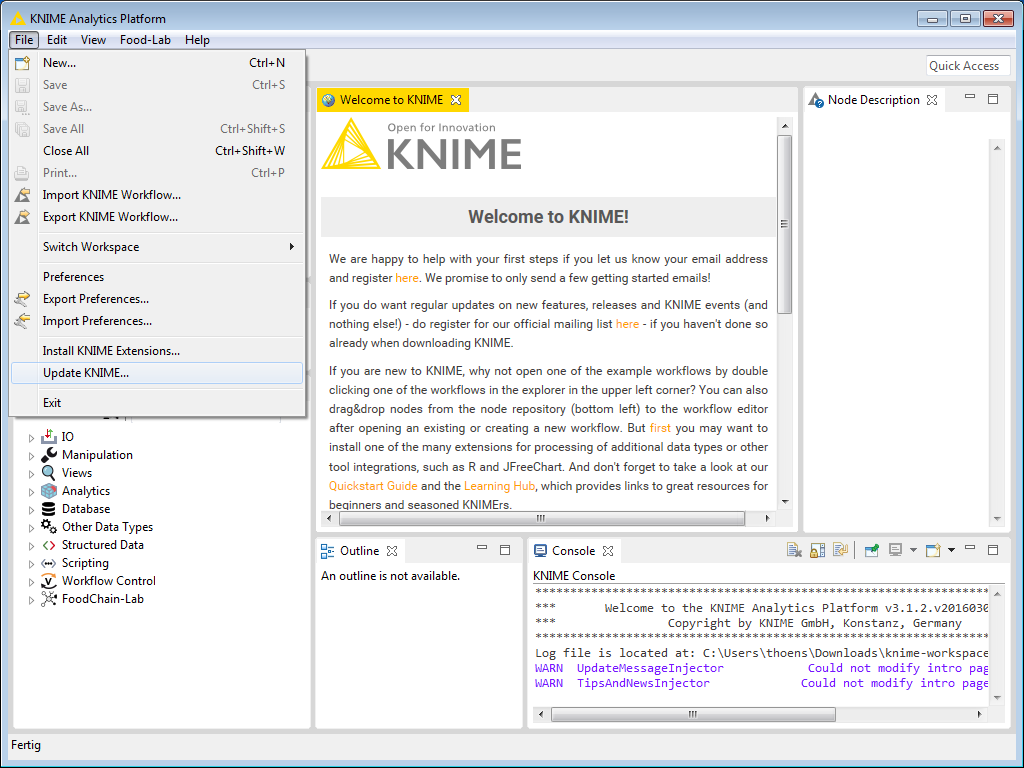
\includegraphics[height=0.6\textheight]{1.png}
	\end{center}
	\begin{itemize}
		\item Wählen Sie \textbf{File $>$ Update KNIME...} in der Menüleiste.
	\end{itemize}
\end{frame}

\section{2}
\begin{frame}
	\begin{center}
  		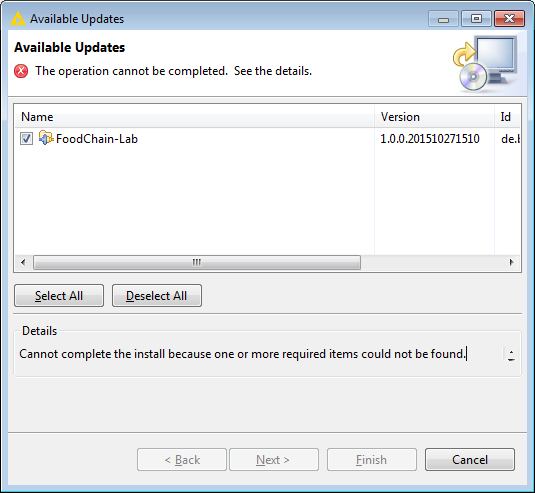
\includegraphics[height=0.6\textheight]{2.png}
	\end{center}
	\begin{itemize}
		\item Falls es nur für eine KNIME Erweiterung ein Update gibt, werden Sie diesen Dialog sehen.
		\item Klicken Sie \textbf{Finish} und fahren Sie mit Schritt 6 fort.
		\item Andernfalls (falls mehrere Updates verfügbar sind) fahren Sie mit Schritt 3 fort.
	\end{itemize}
\end{frame}

\section{3}
\begin{frame}
	\begin{center}
  		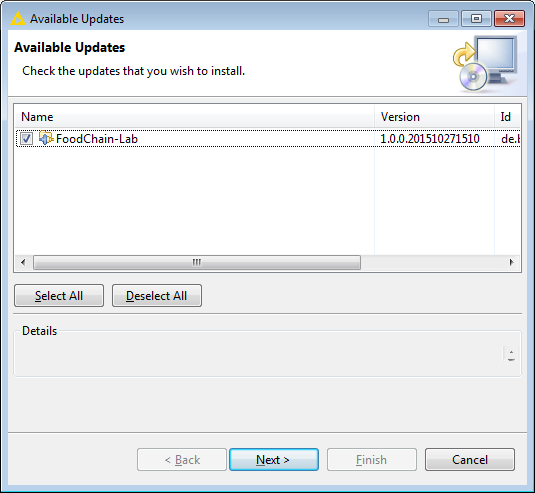
\includegraphics[height=0.6\textheight]{3.png}
	\end{center}
	\begin{itemize}
		\item In diesem Dialog werden all KNIME Erweiterungen gelistet, für die ein Update verfügbar ist.
		\item Stellen Sie sicher, dass alle Einträge ausgewählt sind und klicken Sie \textbf{Next}.
	\end{itemize}
\end{frame}

\section{4}
\begin{frame}
	\begin{center}
  		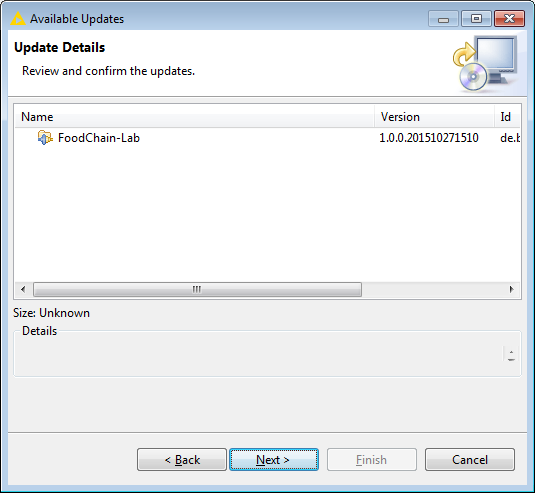
\includegraphics[height=0.6\textheight]{4.png}
	\end{center}
	\begin{itemize}
		\item Im folgenden Installationsmenü wird noch einmal aufgeführt, was nun installiert werden kann. Klicken Sie auf \textbf{Next}.
	\end{itemize}
\end{frame}

\section{5}
\begin{frame}
	\begin{center}
  		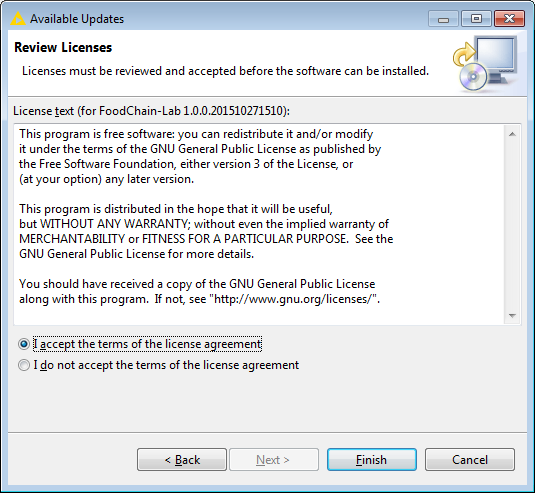
\includegraphics[height=0.6\textheight]{5.png}
	\end{center}
	\begin{itemize}
		\item Lesen und akzeptieren Sie die Lizenzvereinbarung und klicken Sie anschließend auf \textbf{Finish}.
	\end{itemize}
\end{frame}

\section{6}
\begin{frame}
	\begin{center}
  		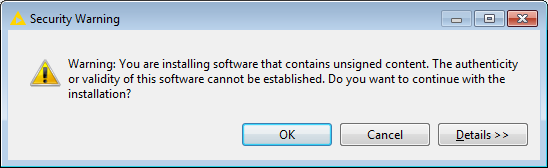
\includegraphics[width=0.7\textwidth]{6.png}
	\end{center}
	\begin{itemize}
		\item Sollten Sie eine Sicherheitswarnung erhalten, weil die Authentizität oder Validität der Software nicht ermittelt werden kann, klicken Sie bitte auf \textbf{OK}.
	\end{itemize}
\end{frame}

\section{7}
\begin{frame}
	\begin{center}
  		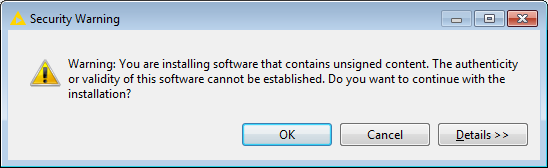
\includegraphics[width=0.7\textwidth]{7.png}
	\end{center}
	\begin{itemize}
		\item Nach der Installation starten Sie bitte KNIME neu (klicken Sie auf \textbf{Restart}).
	\end{itemize}
\end{frame}

\end{document}